\section{Paths in Graphs}

	\subsection{Single Source Shortest Path (SSSP)}
	\begin{itemize}
		\item We want to compute the distances from a source $s \in V$ to other nodes in $V$. 
		\item We don't use DFS here because DFS might explore much longer paths first, so it might be very 
			inefficient.
		\item Solution: use \textbf{Breadth-First Search (BFS)}
			\begin{itemize}
				\item Analogous to a bird's eye perspective, where we explore successively outward in 
					``neighbourhoods.''
				\item Start at exploring from distance 1, then when everything at distance 1 is explored, 
					continue to explore at distance 2, etc. 
			\end{itemize}
		\item The type of BFS that we use depends a lot on what kind of graph we're dealing with:
			\begin{itemize}
				\item Unweighted graphs: Ordinary BFS works
				\item Positive Weights: Dijkstra's algorithm
				\item Negative Weights allowed: Bellman-Ford Algorithm
			\end{itemize}
		\item Going down this list makes the graph more general, but they are less efficient than the ones 
			above. 

			\question{Would a more correct statement be that BFS works if all the edges have the same weight?}
	\end{itemize}

	\subsection{Breadth First Search (BFS)}
	\begin{itemize}
		\item Start at $s$, and add all the neighbours of $s$ to a queue. For every vertex in 
			the queue, we visit all the unvisited nodes from that vertex, and add it to the queue. Repeat
			until all nodes have been visited.
	\end{itemize}

	\subsubsection{Runtime of BFS}
	\begin{itemize}
		\item 	We enqueue and deque every node exactly once if the node is connected, otherwise we don't do it 
			at all. This takes $O(1)$ time. 
		\item Once an item is dequeued, we need to check all the neighbours of a graph, costing $O(\deg(u))$ 
			time.
		\item In total, our runtime is:
			\[
				\sum_{u \in V} O(1 + \deg(u)) = O(n + m)
			\] 
			This is the same runtime as DFS, which is not a coincidence! DFS and BFS are actually related, 
			except the queue is replaced by a stack.
		\item We didn't implement it as a stack in lecture, but the idea is the same.
	\end{itemize}

	\subsection{Weighted Graphs}
	\begin{itemize}
		\item BFS doesn't work here because it ignores the weights of the graph. It is possible that a graph 
			ends up being shorter but goes through more nodes, a possibility that BFS doesn't catch.
		\item \textbf{Useful Fact:} Any sub path of a shortest path is also a shortest path. This is rather 
			obvious.
		\item So what we should think about is that to build the shortest path, we build the shortest path from 
			other, shotest paths but add in the shortest edge. This guarantees that our shortest path 
			remains the shortest.
	\end{itemize}

	\subsection{Dijkstra's Algorithm}
	\begin{itemize}
		\item Let $K$ denote the set of ``known'' nodes where the length of shortest path is computed. To 
			determine node we should add to $K$, we should select the vertex that gives the smallest 
			$\dist(s, u) + \ell(u, v)$. Visually:
			\begin{center}
				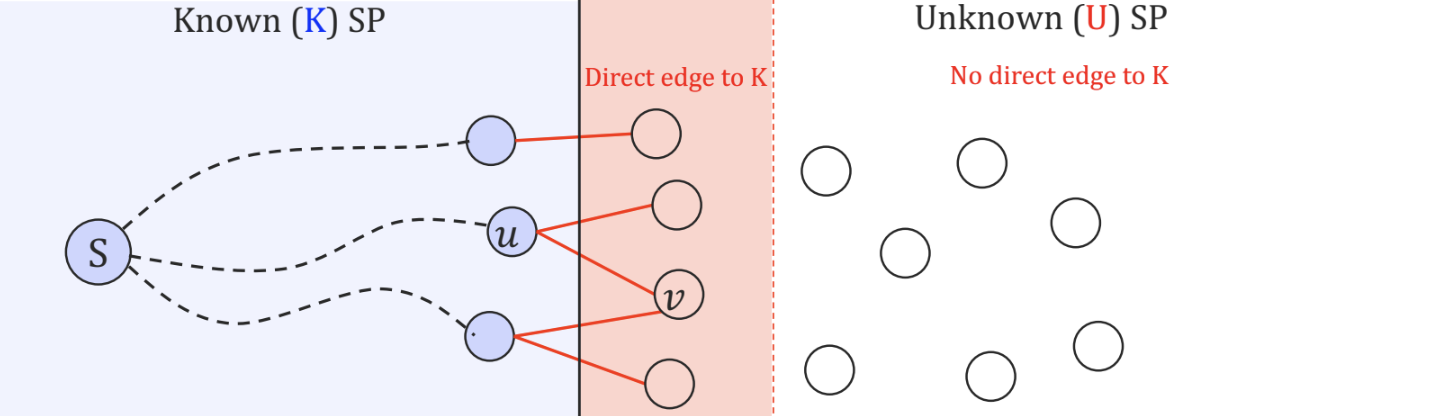
\includegraphics[scale=0.5]{dijkstra.png}
			\end{center}
		\item The red region is the set of nodes that we look at.
		\item We don't need to recompute all distances at every iteration - instead we can just store 
			the distances as we go along. Initial overestimates are fine, since eventually we will explore 
			the shortest path, and its distance will eventually be updated. 
		\item If we find a shorter path later on, we can update $\dist(s, u)$ to reflect that.
		\item If we want to find the shortest path from $S$, then we can add a new variable that stores 
			the previous node in the sequence from $S$ to $u$. Therefore, when we want to find the 
			shortest path, then we are continually looking backward until we get back to $S$. 
	\end{itemize}

	\subsubsection{Runtime of Dijkstra's}
	\begin{itemize}
		\item The runtime of Dijkstra's depends on the kind of data structure we used to keep track 
			of the distances:
			\begin{center}
				\begin{tabular}{c|c|c|c|c}
					\textbf{Implementation} & \textbf{Insert} & \textbf{Delete Min} & 
					\textbf{Decrease Key} & \textbf{Runtime}\\
					\hline 
					Array & $O(1)$ & $O(n)$ & $O(1)$ & $O(n^2 + m) = O(n^2)$\\
					Binary Heap & $O(\log n)$ & $O(\log n)$ & $O(\log n)$ & $O((n + m) \log n)$\\
					Fibonacci Heap & $O(1)$ & $O(\log n)$ & $O(1)$ & $O(n \log n + m)$
				\end{tabular}
			\end{center}
		\item The best known runtime of Dijkstra's algorithm is $O(n \log \log n + m)$.
		\item At the end of the day, this is slower than DFS, by the $\log n$ term.
	\end{itemize}
	
	\subsection{Negative Weights: Bellman-Ford Algorithm}
	\begin{itemize}
		\item Sometimes, having negative weights is possible, for instance when traversing an edge is more 
			beneficial to you in some way.
		\item Shortest paths don't really make sense if a cycle has negative length (since then we'd be 
			infinitely descending) 
		\item All we need to do is modify Dijkstra's update function!
			\begin{itemize}
				\item Call an update ``safe'' if $\dist(w)$ is an overestimate of the true shortest path 
					between $s$ and $w$. In other words, $\dist(w) \ge d(s, w)$ for all $w \in V$. 
			\end{itemize}
	\end{itemize}

	\question{see lectures for Bellman-Ford}
